
\section{Poprzedni wykład- ciąg dalszy}
Jak już pokazano, funkcja Wignera jest zdefiniowana poprzez transformate Wignera:
\begin{equation}\varrho_w(\R,\P,t)=\frac{1}{(2\pi\hbar)^3}
\int d^3S\varrho(\R+\frac{1}{2}\S,\R-\frac{1}{2}\S,t)e^{-\frac{i}{\hbar}\P\cdot\S}
\end{equation}
Funkcja ta pojawiła się w równaniu ruchu dla układu statystycznego, czyli równaniu ruchu dla funkcji Wignera:
\begin{equation}i\hbar\frac{d}{dt}\hat{\varrho}(t)=\Big[\hat{H},\hat{\varrho}(t)\Big]
\end{equation}
Rozpiszmy powyższy komutator:
\begin{equation}i\hbar\frac{d}{dt}\hat{\varrho}(t)=\hat{H}\hat{\varrho}(t)-\hat{\varrho}(t)\hat{H}=\hat{H}\mathds{1}\hat{\varrho}(t)-\hat{\varrho}(t)\mathds{1}\hat{H}
\end{equation}
i wybierzmy reprezentację położeniową, w której ogólnie:
\begin{equation}
\langle r'|\hat{\varrho}(t)|\r\rangle=\varrho(\r',\r,t)
\end{equation}
zatem w naszym równaniu, po wykorzystaniu zupełności bazy:
\begin{equation}i\hbar\partial_t\varrho(\r',r,t)=
\int d^3r''\Big(H(\r',\r'')\varrho(\r'',r,t)-
\varrho(\r',\r'',t)H(\r'',r)\Big)
\end{equation}
\subsection{Wyprowadzenie równania ruchu Wignera}
\subsubsection{Równanie von Neumanna w przybliżeniu jednocząstkowym i lokalnym}
Zastosujemy następujące przybliżenia:
\begin{itemize}
\item[1.] Przybliżenie lokalne:
\begin{equation}H(\vec{\xi},\vec{\xi}')=H(\vec{\xi})\delta(\vec{\xi}-\vec{\xi}\,')
\end{equation}
\item[2.] Przyjmujemy, że hamiltonian jest operatorem jednocząstkowym:
\begin{equation}H(\vec{\xi})=-\frac{\hbar^2}{2m}\nab{\vec{\xi}}^2+U(\vec{\xi})
\end{equation}
\end{itemize}
Równanie ruchu dla funkcji Wignera w tych przybliżeniach ma następującą postać:
\begin{equation}i\hbar\partial_t\varrho(\r',r,t)=
\int d^3r''\Big(H(\r')\delta(\r'-\r'')\varrho(\r'',r,t)-
\varrho(\r',\r'',t)H(\r'')\delta(\r''-\r)\Big)
\end{equation}
Z twierdzenia filtracyjnego o delcie Diraca:
\begin{equation}i\hbar\partial_t\varrho(\r',r,t)=
\Big(H(\r')\varrho(\r',r,t)-
\varrho(\r',\r,t)H(\r)\Big)
\end{equation}
\begin{equation}i\hbar\partial_t\varrho(\r',r,t)=
\Big(H(\r')-H(\r)\Big)\varrho(\r',r,t)
\end{equation}
Obliczenia wykonamy w jednym wymiarze:
\begin{equation}\r'\rightarrow x'~~~~~~~~~~\r\rightarrow x\end{equation}
zatem:
\begin{equation}i\hbar\underbrace{\partial_t\varrho(x',x,t)}_{\text{szybkość zmian} \varrho}=
\underbrace{-\frac{\hbar^2}{2m}\Big(\frac{\partial^2}{\partial x'^2}-\frac{\partial^2}{\partial x^2}\Big)\varrho(x',x,t)}_{\text{człon kinetyczny}}
+\underbrace{\Big(U(x')-U(x)\Big)\varrho(x',x,t)}_{\text{człon potencjalny}}
\label{vonNeumann}
\end{equation}
Jest to tzw. \textbf{równanie von Neumanna w przybliżeniu jednocząstkowym i lokalnym.}\\
\subsubsection{Wprowadzenie nowych zmiennych i transformata Fouriera}
Tak jak na poprzednich wykładach, wprowadzamy nowe zmienne:
\begin{equation}\begin{cases} R=\frac{1}{2}(x'-x)\\ S=x'-x \end{cases} \Rightarrow  \begin{cases}  x'=R+\frac{1}{2}S\\ x=R-\frac{1}{2}S\end{cases}
\end{equation}
Następnie do równania (\ref{vonNeumann}) trzeba wprowadzić nowe zmienne i zastosować transformację Fouriera. Czynności te wykonamy dla kolejnych członów osobno.
\begin{itemize}
\item Wyraz odpowiadający za szybkość zmian macierzy gęstości\\
Przeprowadzamy do nowych zmiennych:
\begin{equation}i\hbar\partial_t\varrho(x',x,t)=
i\hbar\partial_t\varrho(R+\frac{1}{2}S,R-\frac{1}{2}S,t)
\end{equation}
i wykonujemy transformację Fouriera:
\begin{equation}
i\hbar\partial_t\frac{1}{2\pi\hbar}\int dS\varrho(R+\frac{1}{2}S,R-\frac{1}{2}S,t) 
e^{-\frac{i}{\hbar}PS}=i\hbar\partial_t\varrho_w(R,P,t)
\end{equation}
\item Wyraz kinetyczny
\begin{equation}
-\frac{\hbar^2}{2m}\Big(\frac{\partial^2}{\partial x'^2}-\frac{\partial^2}{\partial x^2}\Big)\varrho(x',x,t)
\end{equation}
Przeprowadzamy do nowych zmiennych pochodną z reguły łańcuchowej:
\begin{equation}\frac{\partial}{\partial x'}=
\frac{\partial}{\partial R}\frac{\partial R}{\partial x'}+
\frac{\partial}{\partial S}\frac{\partial S}{\partial x'}=
\frac{1}{2}\frac{\partial}{\partial R}+
\frac{\partial}{\partial S}=
\frac{1}{2}\partial_R+
\partial_S
\end{equation}
\begin{equation}\frac{\partial}{\partial x}=
\frac{\partial}{\partial R}\frac{\partial R}{\partial x}-
\frac{\partial}{\partial S}\frac{\partial S}{\partial x}=
\frac{1}{2}\frac{\partial}{\partial R}-
\frac{\partial}{\partial S}=
\frac{1}{2}\partial_R-
\partial_S
\end{equation}
Podobnie pochodne drugiego rzędu:
\begin{equation}\frac{\partial^2}{\partial x'^2}=
\frac{1}{2}\frac{\partial}{\partial R}\Big(\frac{1}{2}\frac{\partial}{\partial R}+
\frac{\partial}{\partial S}\Big)+
\frac{\partial}{\partial S}\Big(\frac{1}{2}\frac{\partial}{\partial R}+
\frac{\partial}{\partial S}\Big)=\frac{1}{4}\partial_R^2+
\partial_S^2+{\partial_{RS}^2}
\end{equation}
gdzie zakładamy, że pochodne cząstkowe są przemienne:
\begin{equation}
\partial_{RS}^2\equiv=\frac{\partial}{\partial S}\frac{\partial}{\partial R}=\frac{\partial}{\partial R}\frac{\partial}{\partial S}
\end{equation}
Analogicznie:
\begin{equation}\frac{\partial^2}{\partial x^2}=
\frac{1}{4}\partial_R^2+
\partial_S^2-{\partial_{RS}^2}
\end{equation}
Zatem człon kinetyczny w nowych zmiennych to:
\begin{equation}
-\frac{\hbar^2}{2m}\Big(\frac{\partial^2}{\partial x'^2}-\frac{\partial^2}{\partial x^2}\Big)\varrho(x',x,t)=
-\frac{\hbar^2}{2m}\Big(\frac{1}{4}\partial_R^2+
\partial_S^2+{\partial_{RS}^2}-\frac{1}{4}\partial_R^2-
\partial_S^2+{\partial_{RS}^2}\Big)\varrho(R+\frac{1}{2}S,R-\frac{1}{2}S,t)=
\nonumber
\end{equation}
\begin{equation}
=-\frac{\hbar^2}{m}\partial_{RS}^2\varrho(R+\frac{1}{2}S,R-\frac{1}{2}S,t)
\end{equation}
Transformata Fouriera z tego wyrażenia to:
\begin{equation}
-\frac{\hbar^2}{m}\frac{1}{2\pi\hbar}\int dS \partial_{RS}^2\varrho(R+\frac{1}{2}S,R-\frac{1}{2}S,t)e^{-\frac{i}{\hbar}PS}=\nonumber
\end{equation}
Zastąpimy $\varrho$ jej odwrotną transformatą Fouriera:
\begin{equation}
=-\frac{\hbar^2}{m}\frac{1}{2\pi\hbar}\partial_R\int dS \partial_S\Big\lbrace
\int dP'\varrho_w(R,P',t)e^{\frac{i}{\hbar}P'S}\Big\rbrace e^{-\frac{i}{\hbar}PS}=
\nonumber
\end{equation}
Następnie obliczymy pochodną cząstkową po $S$ i przeszeregujemy równanie:
\begin{equation}
=-\frac{\hbar^2}{m}\frac{i}{\hbar}\partial_R\int dP'\varrho_w(R,P',t)
\underbrace{\frac{1}{2\pi\hbar}
\int dS \partial_S P'
e^{\frac{i}{\hbar}(P'-P)S}}_{\delta(P'-P)}=
\nonumber
\end{equation}
\begin{equation}
=-\frac{i\hbar}{m}\partial_R\int dP'\varrho_w(R,P',t)P'\delta(P'-P)=
\nonumber
\end{equation}
\begin{equation}
=-\frac{i\hbar}{m}\partial_R P\varrho_w(R,P,t)
\end{equation}
\item Wyraz potencjalny\\
Wyrażamy go w nowych zmiennych:
\begin{equation}
\Big(U(x')-U(x)\Big)\varrho(x',x,t)=
\Big(U(R+\frac{1}{2}S)-U(R-\frac{1}{2}S)\Big)\varrho(R+\frac{1}{2}S,R-\frac{1}{2}S,t)
\end{equation}
i przeprowadzamy transformację Fouriera:
\begin{equation}\frac{1}{2\pi\hbar}\int dS\Big(U(R+\frac{1}{2}S)-U(R-\frac{1}{2}S)\Big)\varrho(R+\frac{1}{2}S,R-\frac{1}{2}S,t)e^{-\frac{i}{\hbar}PS}=
\nonumber
\end{equation}
Zastępujemy $\varrho$ jej odwrotną transformatą Fouriera:
\begin{equation}=\frac{1}{2\pi\hbar}\int dS\Big(U(R+\frac{1}{2}S)-U(R-\frac{1}{2}S)\Big)
\int dP'\varrho_w(R,P',t)e^{\frac{i}{\hbar}P'S}e^{-\frac{i}{\hbar}PS}=
\nonumber
\end{equation}
Następnie przeszeregujemy to równanie oraz dodamy do licznika i mianownika czynnik $i\hbar$, ponieważ znalazł się on w liczniku transformaty Fouriera poprzednich członów- tego odpowiedzialnego za szybkość zmian macierzy gęstości i członu kinetycznego.
\begin{equation}=\frac{i\hbar}{2\pi \hbar}\int dP'
\Big\lbrace \underbrace{
\frac{1}{i\hbar}\int dS\Big(U(R+\frac{1}{2}S)-U(R-\frac{1}{2}S)\Big)
e^{\frac{i}{\hbar}(P'-P)S}}_{U_w(R,P'-P)}
\Big\rbrace
\varrho_w(R,P',t)=
\nonumber
\end{equation}
\begin{equation}=\frac{i\hbar}{2\pi \hbar}\int dP'
U_w(R,P'-P)
\varrho_w(R,P',t)
\end{equation}
Przez $U_w(R,P'-P)$ oznaczono tzw. \textbf{potencjał Wignera}. Należy zauważyć, że potencjał ten jest nielokalny (bo występuje w nim całka $\int dS$, która "zbiera" informacje z całej przestrzeni, bo $S=x'-x$).
\end{itemize}
\subsubsection{Podsumowanie- wyprowadzenie równania ruchu Wignera}
Ostatecznie więc równanie (\ref{vonNeumann}) przechodzi w:
\begin{equation}
i\hbar\partial_t\varrho_w(R,P,t)=
-\frac{i\hbar}{m}\partial_R P\varrho_w(R,P,t)
+\frac{i\hbar}{2\pi \hbar}\int dP' U_w(R,P'-P) \varrho_w(R,P',t)
\end{equation}
\begin{equation}
\partial_t\varrho_w(R,P,t)
+\frac{P}{m}\partial_R \varrho_w(R,P,t)
=\frac{1}{2\pi \hbar}\int dP' U_w(R,P'-P) \varrho_w(R,P',t)
\label{rWignera}
\end{equation}
W trzech wymiarach powyższe równanie przechodzi w:
\begin{equation}
\partial_t\varrho_w(\R,\P,t)+\vec{v}(\p)\partial_R \varrho_w(\R,\P,t)
=\frac{1}{(2\pi \hbar)^3}\int d^3P' U_w(\R,\P'-\P) \varrho_w(\R,\P',t)
\end{equation}
Jest to tzw. \textbf{równanie ruchu Wignera}.\\
Zauważmy, że to równanie jest podobne do równania Boltzmanna, przy czym lewa strona równania podobna jest do części kinetycznej, a prawa- do części potencjalnej równania Boltzmanna.\\
Równanie ruchu Wignera różni się od równania Boltzmanna w sposób następujący:
\begin{itemize}
\item w równaniu Boltzmanna rozkład jest klasyczny- jest to funkcja rozkładu gęstości. W równaniu Wignera rozkład jest kwantowy- jest to macierz gęstości.
\item w równaniu Wignera potencjał jest nielokalny (a w równaniu Boltzmanna- lokalny)
\end{itemize}
\subsection{Doprowadzenie równania ruchu Wignera do postaci rozwiązywalnej numerycznie}
Załóżmy, że potencjał daje się podzielić na potencjał wewnętrzny (odpowiedzialny za wewnętrzną strukturę układu) oraz potencjał zewnętrzny:
\begin{equation}U(x)=U_{int}(x)+U_{ext}(x)
\end{equation}
Przy czym:
\begin{equation}U_{ext}(x)=-exE\end{equation}
Zatem zewnętrzny potencjał Wignera:
\begin{equation}
U_w^{ext}(R,P'-P)=\frac{1}{i\hbar}\int dS \big[ e(R+\frac{1}{2}S)E+e(R-\frac{1}{2}S)E \big]e^{\frac{i}{\hbar}(P'-P)S}
\end{equation}
Po uporządkowaniu:
\begin{equation}
U_w^{ext}(R,P'-P)=-\frac{eE}{i\hbar}\underbrace{\int dS Se^{-\frac{i}{\hbar}(P-P')S}}_{I} \label{w13r1}
\end{equation}
Zauważmy, że
\begin{equation}
\partial_P e^{-\frac{i}{\hbar}(P-P')S}=-\frac{i}{\hbar}Se^{-\frac{i}{\hbar}(P-P')S}
\end{equation}
Zatem:
\begin{equation}
Se^{-\frac{i}{\hbar}(P-P')S}=i\hbar\partial_P e^{-\frac{i}{\hbar}(P-P')S}
\end{equation}
\begin{equation}
 I=\int dS Se^{-\frac{i}{\hbar}(P-P')S}=
 i\hbar\partial_P \int dS e^{-\frac{i}{\hbar}(P-P')S}\frac{2\pi\hbar}{2\pi\hbar}=
 \nonumber
 \end{equation}
 \begin{equation}
= i\hbar\cdot 2\pi\hbar\partial_P\delta(P-P')
 \end{equation}
 Stąd równanie (\ref{w13r1}) przechodzi w:
 \begin{equation}
 U_w^{ext}(R,P'-P)=-\frac{eE}{i\hbar}i\hbar\cdot 2\pi\hbar\partial_p\delta(P-P')
 \end{equation}
 Zatem równanie ruchu Wignera (\ref{rWignera}) w jednym wymiarze można przepisać jako:
\begin{equation}
\partial_t\varrho_w(R,P,t)+
v\partial_R \varrho_w(R,P,t)
=\nonumber
\end{equation}
\begin{equation}=-eE\int dP' \partial_P\delta(P-P') \varrho_w(R,P',t)
+\frac{1}{2\pi\hbar}\int dP' U_w^{int}(R,P'-P)\varrho_w(R,P',t)
\end{equation}
Korzystając z twierdzenia filtracyjnego o delcie Diraca:
\begin{equation}
\partial_t\varrho_w(R,P,t)+
v\partial_R \varrho_w(R,P,t)+eE\partial_P \varrho_w(R,P,t)=
\frac{1}{2\pi\hbar}\int dP' U_w^{int}(R,P'-P)\varrho_w(R,P',t)
\end{equation}
Zauważmy, że lewa strona równania przypomina równanie Boltzmanna w polu elektrycznym, natomiast prawa strona to całka zderzeń spowodowanych wewnętrzną strukturą układu. 
Oczywiście w równanie to nadal różni się od równania Boltzmanna przez kwantowy (a nie klasyczny) rozkład gęstości oraz przez nielokalny potencjał. Dlatego równanie ruchu Boltzmanna często nazywa się \textbf{kwantowym równaniem Boltzmanna z nielokalnym potencjałem.}\\
Powyższe równanie wraz z równaniami opisującymi:
\begin{itemize}
\item koncentrację:
\begin{equation}
n(R,t)=\int dP \varrho(R,P,t)
\end{equation}
\item gęstość prądu:
\begin{equation}
j(R,t)=\int dP v(P) \varrho(R,P,t)
\end{equation}
\item równanie Poissona
\begin{equation}
\partial_R E(R)=e\Big[n(R,t)-N_D(R)\Big]
\end{equation}
gdzie $N_D$ to koncentracja donorów
\end{itemize}
tworzą układ równań, który rozwiązuje się numerycznie w cyklu samouzgodnionym. W ten sposób uzyskuje się zależność $j(E)$. Obecnie powyższe równanie rozwiązano co najwyżej w dwóch wymiarach.\\
\subsection{Przybliżenie lokalne potencjału Wignera a równanie Boltzmanna}
 Potencjał Wignera, jak pokazano wyżej, ma postać:
\begin{equation}U_w(R,P'-P)=\frac{1}{i\hbar}\int dS\Big[ U(R+\frac{1}{2}S)-U(R-\frac{1}{2}S)\Big] e^{\frac{i}{\hbar}(P'-P)S}\label{UW}
\end{equation}
\subsubsection{Co to oznacza, że potencjał jest nielokalny?}
Oznacza to, że na ołówek, który trzymamy w ręce ma wpływ szydełkowanie sąsiadki.\\ Podobnym efektem jest\textbf{ efekt Aharonova-Bohma}. Jest to kwantowo-mechaniczny efekt, potwierdzony doświadczalnie. Polega on na tym, że kiedy umieścimy elektron na pierścieniu i wytworzymy pole magnetycznym w punkcie, w którym nie ma elektronu, to i tak ten elektron czuje to pole magnetyczne.
\begin{center}
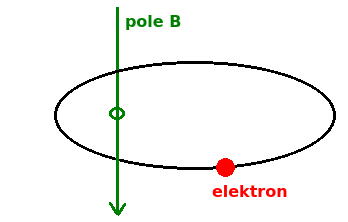
\includegraphics[scale=0.5]{obrazki/wykl_13_obrazek1.png}
\end{center}
 Dzieje się tak, ponieważ elektron w istocie czuje związany z polem magnetycznym potencjał wektorowy, który jest w całej przestrzeni. Swoją drogą, efekt ten udowadnia, że w mechanice kwantowej fizyczne jest nie tylko pole np. magnetyczne (jak to było w mechanice klasycznej), ale również potencjał.\\
\subsubsection{Przybliżenie lokalne potencjału Wignera}
Rozwińmy potencjał w szereg:
\begin{equation}U(R\pm\frac{1}{2}S)=U(R)\pm \frac{1}{2}U'(R)S+...+\mathcal{O}(S^2)
\end{equation}
Przybliżenie lokalne:
\begin{equation}U(R\pm\frac{1}{2}S)\simeq U(R)\pm \frac{1}{2}U'(R)S
\end{equation}
Zatem, po wykonaniu dodawania w potencjale Wignera (\ref{UW}), potencjał Wignera w przybliżeniu lokalnym przedstawia się wzorem:
\begin{equation}
U_w(R\pm\frac{1}{2}S)\simeq
\frac{1}{i\hbar}\int dS \partial_R U(R) Se^{\frac{i}{\hbar}(P'-P)S}=\nonumber
\end{equation}
\begin{equation}
=\frac{1}{i\hbar}\partial_R U(R)\int dS Se^{\frac{i}{\hbar}(P'-P)S}
\end{equation}
Całkę powyższą już obliczaliśmy poprzednio. Kopiując ówczesne rozwiązanie, dostajemy:
\begin{equation}
U_w(R\pm\frac{1}{2}S)\simeq \partial_R U(R)\frac{1}{i\hbar}i\hbar 2\pi\hbar \partial_P \delta(P-P')=2\pi\hbar\partial_R U(R) \partial_P \delta(P-P')
\end{equation}
Zatem równanie Wignera w przybliżeniu lokalnym ma postać:
\begin{equation}
\partial_t\varrho_w(R,P,t)+
v\partial_R \varrho_w(R,P,t)=
\frac{2\pi\hbar}{2\pi\hbar}\int dP' \partial_R U(R) \partial_P \delta(P-P')\varrho_w(R,P',t)
\end{equation}
Wykorzystując twierdzenie filtracyjne o delcie Diraca:
\begin{equation}
\partial_t\varrho_w(R,P,t)+
v\partial_R \varrho_w(R,P,t)\underbrace{-
 \partial_R U(R)}_{\text{siła F}} \partial_P \varrho_w(R,P,t)=0
\end{equation}
Ostatecznie:
\begin{equation}
\partial_t\varrho_w(R,P,t)+
v\partial_R \varrho_w(R,P,t)+F \partial_P \varrho_w(R,P,t)=0
 \end{equation}
 Zauważmy, że jest to dokładne równanie Boltzmanna w polu siły F, z tą różnicą, że zamiast funkcji rozkładu gęstości mamy macierz gęstości (czyli mamy rozkład kwantowy zamiast klasycznego).\\
Sytuację tę można pokazać jako Gaussian poruszający się po trajektorii klasycznej wyznaczonej z równania Boltzmanna:
\begin{center}
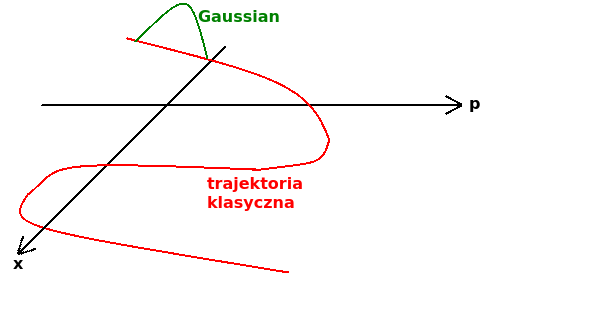
\includegraphics[scale=0.5]{obrazki/wykl_13_obrazek2.png}
\end{center}
Gaussian ten przy poruszaniu rozciąga się i kurczy. Aby to wyjaśnić, można sobie wyobrazić, że w chwili $t=0$ rzuten Gaussianu na płaszczyznę we współrzędnych położenie-pęd jest okrąg. W następnych chwilach pęd jest większy dla większych x (ponieważ dla nich większa jest prędkość) i mniejszy dla mniejszych x- w ten sposób okrąg zamienia się w "cygaro":
\begin{center}
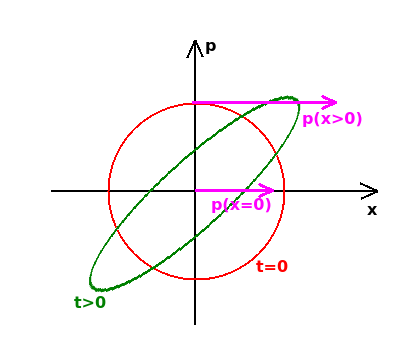
\includegraphics[scale=0.5]{obrazki/wykl_13_obrazek3.png}
\end{center}

\section{Wstęp do nierównowagowych funkcji Greena}
\subsection{Dwuczasowa funkcja korelacji}
Wartość oczekiwana zmiennej dynamicznej wyraża się wzorem:
\begin{equation}\langle A(t)\rangle=Tr\lbrace\hat{A}\hat{\varrho}(t)\rbrace=
Tr\lbrace\hat{\varrho}(t)\hat{A}\rbrace
\end{equation}
gdzie przemienność pod znakiem śladu macierzy jest ogólną własnością śladu macierzy.\\
Operator macierzy gęstości przedstawia się wzorem:
\begin{equation}\hat{\varrho}(t)=\sum_i|\psi_i(t)\rangle\langle\psi_i(t)|=\sum_i\hat{P}_{\psi_i}(t)\end{equation}
gdzie $\hat{P}_{\psi_i}(t)$ to operator rzutowy.
W reprezentacji $\alpha$:
\begin{equation}\varrho(\vec{\alpha}\,',\vec{\alpha},t)=
\langle \vec{\alpha}\,'|\hat{\varrho}(t)|\vec{\alpha}\rangle=\sum_i \varrho_i\psi_i(\vec{\alpha}\,',t)\psi_i^*(\vec{\alpha},t)
\end{equation}
Zauważmy, że w powyższym wyrażeniu obie funkcje falowe $\psi$ są określone w jednej chwili $t$- a to oznaczałoby, że wszystkie oddziaływania musiałyby być natychmiastowe.\\
Aby tego uniknąć, uogólniamy to wyrażenie na dwie chwile czasowe. W ten sposób dostajemy:
\begin{itemize}
\item elektronową funkcję korelacji
\begin{equation}G^<(\alpha',t';\alpha,t)=
\sum_i\varrho_i\psi_i(\alpha',t')\psi_i^*(\alpha,t)
\end{equation}
Jest to tzw. nierównowagowa funkcja Greena "\textit{G- mniejsze}".\\
Ponadto widzimy, że:
\begin{equation}\varrho(\alpha',\alpha,t)=G^<(\alpha',t';\alpha,t)_{|_{t'=t}}
\end{equation}
\item dziurową funkcję korelacji
\begin{equation}G^>(\alpha',t';\alpha,t)=
\sum_i\varrho_i\psi_i(\alpha,t)\psi_i^*(\alpha',t')
\end{equation}
Jest to tzw. nierównowagowa funkcja Greena "\textit{G- większe}".
\end{itemize}
\subsection{Interpretacja dwupunktowej funkcji korelacji $G^{\lessgtr}$}
W reprezentacji położeniowej:
\begin{itemize}
\item funkcja korelacji $G^<(\r\,',t';\r,t)$ opisuje amplitudę przejścia cząstki wykreowanej w punkcie $\r$ w chwili $t$ i usuniętej w punkcie $\r\,'$ w chwili $t'$ z układu.\\
Ukazuje to poniższy obrazek:
\begin{center}
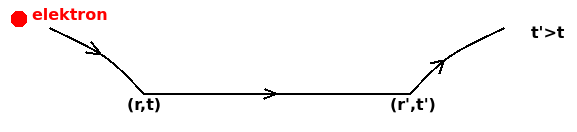
\includegraphics[scale=0.5]{obrazki/wykl_13_obrazek4.png}
\end{center}
Między punktem $(r,t)$ a $(r',t')$ elektron jest "ubrany" w oddziaływania, które są uwzględnione w funkcji korelacji.
\item funkcja korelacji $G^>(\r\,',t';\r,t)$ opisuje amplitudę przejścia cząstki wykreowanej w punkcie $\r\,'$ w chwili $t'$ i usuniętej w punkcie $\r$ w chwili $t$ z układu.\\
\begin{center}
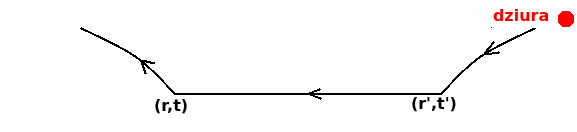
\includegraphics[scale=0.5]{obrazki/wykl_13_obrazek5.png}
\end{center}
Jak widać, jest to zjawisko odwrotne do $G^<$, co więcej- zjawisko to dzieje się wstecz w czasie. Stąd wniosek, że zjawisko to dotyczy przeciwieństwa elektronu, czyli dziury.
\end{itemize}
\subsection{Funkcja $G^<$ a funkcja Wignera}
Dlaczego potrzebujemy funkcji $G^<$?\\
Ponieważ wyrażają się przez nią:
\begin{itemize}
\item Gęstość ładunku
\begin{equation}\rho(\r\,',t)\equiv n(\r\,',t)=-i\hbar G^<(\r\,',t;\r\,',t)
\end{equation}
\item Gęstość prądu
\begin{equation}j(\r\,',t)=\frac{\hbar^2}{2m}\lim_{\r\rightarrow \r\,'}
\Big[\nab{\r}-\nab{\r\,'}\Big] G^<(\r\,',t;\r,t)
\end{equation}
\end{itemize}
Dowolną funkcję $F(\r\,',t';\r,t)$ można przedstawić w nowych zmiennych:
\begin{equation}
\begin{cases}
\R=\frac{1}{2}(\r\,'+\r)\\
\S=r'-\r\\
T=\frac{1}{2}(t'+t)\text{~~- opisuje powolne zmiany spowodowane zewnętrznym polem}\\
\tau=t'-t\text{~~- opisuje szybkie zmiany spowodowane zewnętrznym polem}\\
\end{cases}
\end{equation}
W szczególności przedstawimy tak funkcję \textit{G-mniejsze}:
\begin{equation}
G^<\Big(\R+\frac{1}{2}\S,T+\frac{1}{2}\tau;\R-\frac{1}{2}\S,T-\frac{1}{2}\tau\Big)
\end{equation}
Wykonajmy podwójną transformację Fouriera na tej funkcji:
\begin{equation}
G^<\Big(\R,\vec{P},T,\omega\Big)=\frac{1}{(2\pi\hbar)^3}
\int d^3S\int_{-\infty}^{\infty} G^<\Big(\R+\frac{1}{2}\S,T+\frac{1}{2}\tau;\R-\frac{1}{2}\S,T-\frac{1}{2}\tau\Big)e^{-\frac{i}{\hbar}\vec{P}\cdot S}e^{i\omega t}
\end{equation}
Zauważmy, że
\begin{equation}lim_{\tau\rightarrow 0} G^<(\R,\vec{P},T,\omega)=\varrho_w(\R,\vec{P},t)
\end{equation}
przy czym warunek ${\tau\rightarrow 0}$ oznacza, że $t\rightarrow t'$.\\
Widzimy zatem, że funkcja korelacji $G^<$ jest\textbf{ uogólnioną nierównowagową funkcją rozkładu.}
\subsection{Równania Kadanoffa-Bayma}
Równania te są bardzo trudne w wyprowadzeniu, dlatego podajemy tylko jej postać. Równania te w postaci macierzowej przedstawiają się wzorem:
\begin{equation}
\Big[(\hat{G}_0^{-1}-\hat{U},\hat{G}^<\Big]=
\hat{\Sigma}^{R}\hat{G}^<+\hat{\Sigma}^{<}\hat{G}^A
-\hat{G}^R\hat{\Sigma}^{<}-\hat{G}^<\hat{\Sigma}^{A}
\end{equation}
gdzie:\\
\begin{itemize}
\item $\hat{U}$ to zewnętrzny potencjał jednocząstkowy\\
\item $\hat{G}^R$ to opóźniony operator rezolwenty\\
\item $\hat{G}^A$ to przedwczesny operator rezolwenty\\
\item $\hat{\Sigma}^R$ to opóźniony operator energii własnej\\
\item $\hat{\Sigma}^A$ to przedwczesny operator energii własnej\\
\item $\hat{\Sigma}^<$ to operator energii własnej \textit{sigma-mniejsze}\\
\item $\hat{G}^<$ to swobodny operator rezolwenty.\\\\
\end{itemize}
Równania Kadanoffa-Bayma da się sprowadzić do równania Boltzmanna.

